% !TEX program = pdflatex
% =====================================================================
%  OR CONFERENCE TALK — 15-17 min (20 min slot)
%  Style: based on articulo/presentation.tex (Madrid/whale, 16:9)
%  Content: showcase endurance sweep (static snapshots) + MIQP families
%           (one per slide) + mean-based results (vertex complete,
%           English slides, talk in Spanish.
% =====================================================================
\documentclass[aspectratio=169,10pt]{beamer}

\usetheme{Madrid}
\usecolortheme{whale}
\usefonttheme{professionalfonts}
\setbeamertemplate{navigation symbols}{}
\setbeamertemplate{footline}[frame number]
\setbeamertemplate{blocks}[rounded][shadow=false]

\usepackage[utf8]{inputenc}
\usepackage[T1]{fontenc}
\usepackage[english]{babel}
\usepackage{amsmath,amssymb,mathtools}
\usepackage{booktabs}
\usepackage{graphicx}
\usepackage{animate}
\usepackage{xcolor}
\usepackage{tikz}
\usetikzlibrary{shapes.geometric,arrows.meta,positioning,calc}

\graphicspath{{pictures/}{./}{../}}
\hypersetup{colorlinks=true, linkcolor=blue, citecolor=blue, urlcolor=blue}

% Animation helpers: replay frames if available, else static snapshot.
% Frame dirs are gitignored (anim_frames_*), so compilation never breaks.
\newcommand{\droneAnim}[3]{%
  \IfFileExists{../anim_frames_#1/frame_#2.png}{%
    \animategraphics[loop,autoplay,controls,height=0.75\textheight,keepaspectratio]{2}
      {../anim_frames_#1/frame_}{#2}{#3}%
  }{%
    \IfFileExists{../sweep_results_new/endurance_#1.png}{%
      \includegraphics[height=0.82\textheight,keepaspectratio]{../sweep_results_new/endurance_#1.png}%
    }{%
      \includegraphics[height=0.82\textheight,keepaspectratio]{../sweep_results/endurance_#1.png}%
    }%
  }%
}
\newcommand{\droneAnimGrid}[3]{%
  \IfFileExists{../anim_frames_#1/frame_#2.png}{%
    \animategraphics[loop,autoplay,height=0.25\textheight,keepaspectratio]{2}
      {../anim_frames_#1/frame_}{#2}{#3}%
  }{%
    \IfFileExists{../sweep_results_new/endurance_#1.png}{%
      \includegraphics[height=0.25\textheight,keepaspectratio]{../sweep_results_new/endurance_#1.png}%
    }{%
      \includegraphics[height=0.25\textheight,keepaspectratio]{../sweep_results/endurance_#1.png}%
    }%
  }%
}

% keep display equations compact so each family fits one slide
\setlength{\abovedisplayskip}{4pt}
\setlength{\belowdisplayskip}{4pt}
\setlength{\abovedisplayshortskip}{2pt}
\setlength{\belowdisplayshortskip}{2pt}

% ---------------------------------------------------------------------
\title{Coverage Path Planning}
\subtitle{Impact of Drone Endurance on Multi-Operation Planning}
\author[L. Amorosi, P. Dell'Olmo, J. Puerto, C. Valverde]{%
  Lavinia Amorosi \and Paolo Dell'Olmo \and Justo Puerto \and \textbf{Carlos Valverde}}
\institute[Univ.\ Seville -- Sapienza Rome]{%
  Dept.\ Statistics \& Operations Research, University of Seville\\
  Dept.\ Statistical Sciences, Sapienza University of Rome}
\date[OR 2026]{OR Conference \textperiodcentered\ 15--17\,min talk + Q\&A}

\begin{document}

% =====================================================================
\begin{frame}
  \titlepage
  \vspace{-0.35cm}
  {\scriptsize \centering Joint work: Amorosi -- Dell'Olmo -- Puerto -- Valverde
    \;\textperiodcentered\; Gurobi 11.0 + Python \;\textperiodcentered\; reproducible by seed \par}
\end{frame}

% =====================================================================
%  SHOWCASE (structure of presentation.tex)
% =====================================================================


\begin{frame}{Introduction: the problem}
  \begin{columns}[T,onlytextwidth]
    \begin{column}{0.56\textwidth}
      {\small \textbf{Drone coverage path planning (CPP):}}
      \begin{itemize}
        \item One drone must cover a set of \textbf{disjoint polygonal regions} in the plane
        \item \textbf{Limited battery}: each flight (operation) starts and ends at the depot, where the battery is swapped
        \item Each region can be covered along \textbf{spiral chains at different altitudes}: higher altitude $=$ fewer passes, but less air density and more wind
        \item \textbf{Preemption allowed}: the drone may leave a region unfinished and resume it later
        \item \textbf{New implementation}: entry/exit points placed \emph{anywhere} along the rings, not fixed
      \end{itemize}
      \begin{block}{Objective}
        {\small Minimise \textbf{total distance/time} to cover everything, respecting endurance $W^{\max}$ per operation.}
      \end{block}
    \end{column}
    \begin{column}{0.42\textwidth}
      \centering
      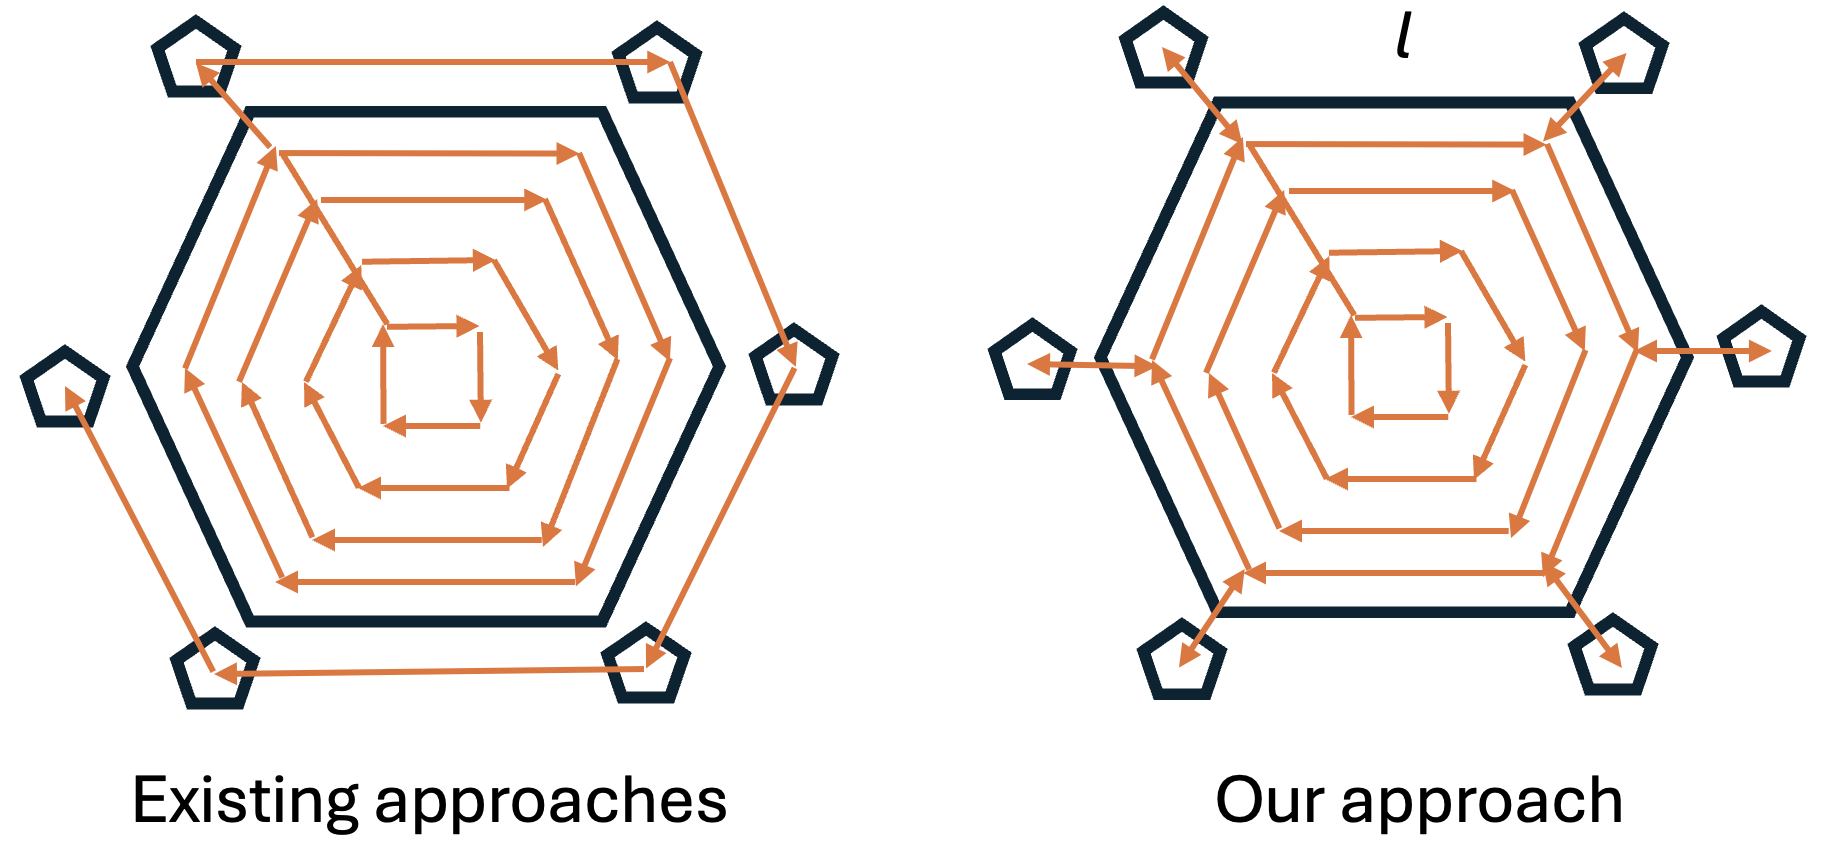
\includegraphics[width=\linewidth]{pictures/Exagon.png}\\
      {\tiny Left: preemption allowed. Right: two-stage (each region in one go). Triangle + 3 satellites: gap $=l/6$. \par}
      \vspace{0.1cm}
      {\scriptsize Applications: aerial inspection, precision agriculture, 3D mapping, disaster response.}
    \end{column}
  \end{columns}
\end{frame}

\begin{frame}{The general problem}
  \begin{columns}[T,onlytextwidth]
    \begin{column}{0.56\textwidth}
      \begin{itemize}
        \item $\mathcal{R}=\{1,\dots,R\}$ disjoint polygonal regions; depot $v_0=(0,0,0)$; endurance $W^{\max}$
        \item Each region $r$: set $\mathcal{T}_r$ of chains, chain $t$ at altitude $h_t$ with segments $\{[Q^s,Q^{s+1}]\}_{s\in\mathcal{S}_t}$
        \item \textbf{Decision}: one chain per region ($\alpha_t$), entry/exit points on it, order of coverage
        \item \textbf{Preemption}: the drone may interrupt a region and resume it later (up to $R-1$ interruptions)
        \item Operations $\mathcal{O}$: tours starting/ending at the depot
      \end{itemize}
      \begin{block}{Feasibility}
        {\footnotesize Every region fits alone in one operation (depot--region--depot $\le W^{\max}$).}
      \end{block}
    \end{column}
    \begin{column}{0.42\textwidth}
      \centering
      
\includegraphics[width=\linewidth]{pictures/set_I.pdf}\\
      {\tiny Candidate points along a chain: start $\mathcal{I}_S$, launch $\mathcal{I}_L$, retrieve $\mathcal{I}_R$, end $\mathcal{I}_T$ \par}
      \vspace{0.1cm}
      {\scriptsize Graph $\mathcal{G}=(\mathcal{V},\mathcal{E})$: intra-chain edges $\mathcal{E}^{int}$, inter-region arcs $\mathcal{E}^{ext}$.}
    \end{column}
  \end{columns}
\end{frame}


\begin{frame}{Decision variables}
  {\small As in the paper, the model has \textbf{four families of constraints}
  \textemdash\ (i) location, (ii) drone path, (iii) distance, (iv) consumption \textemdash\ plus the
  objective (total distance). The main decision variables are:}
  \vspace{0.12cm}
  \begin{columns}[T,onlytextwidth]
    \begin{column}{0.50\textwidth}
      {\small \textbf{Binary and integer:}}
      \begin{itemize}
        \item $\mu_v^{ts}$: vertex $v$ lies on segment $s$ of chain $t$ (location)
        \item $\alpha_t$: chain $t$ is the one selected for its region
        \item $x_{vv'}^o$: the drone traverses $(v,v')$ in operation $o$ (routing)
        \item $y_v^o$: vertex $v$ is visited during operation $o$
        \item $\zeta^o$: everything is covered before operation $o$ starts
        \item $k^o$: number of vertices (or edges) covered in $o$
        \item $\varphi_{rr'},\psi_{rr'}$: inter-region flight altitude and vertical ordering (energy)
      \end{itemize}
    \end{column}
    \begin{column}{0.48\textwidth}
      {\small \textbf{Continuous:}}
      \begin{itemize}
        \item $P_v$: coordinates of vertex $v$ on the selected chain (decision, not input!)
        \item $\gamma_v \in [0,1]$: position of $v$ inside its segment; $\lambda_v$: global chain parametrisation
        \item $dfs_v, efs_v$: cumulative distance / energy from the chain start
        \item $d_{vv'}, d_{vv'}^{xy}, d_{vv'}^{z}$: distance and its horizontal/vertical parts
        \item $w_{vv'}$: energy consumed on $(v,v')$
        \item $\ell_{uv}^o$: linearisation of $x_{uv}^o\cdot d_{uv}$ (objective) and $x_{uv}^o\cdot w_{uv}$ (endurance)
        \item $u_v^o$: position of $v$ in the tour of $o$ (MTZ subtour elimination)
      \end{itemize}
    \end{column}
  \end{columns}
\end{frame}

\begin{frame}{Formulation overview — four families}
  \centering
  {\small Four constraint families + objective (total distance)}\\[0.15cm]
  \begin{columns}[T,onlytextwidth]
    \begin{column}{0.23\textwidth}
      \centering
      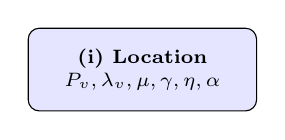
\begin{tikzpicture}[scale=0.62]
        \node[draw, rounded corners, fill=blue!10, minimum width=2.9cm, minimum height=1.05cm, align=center, font=\scriptsize] at (0,0) {\textbf{(i) Location}\\ $P_v,\lambda_v,\mu,\gamma,\eta,\alpha$};
      \end{tikzpicture}
      \\[0.06cm] {\tiny places vertices on segments}
    \end{column}
    \begin{column}{0.23\textwidth}
      \centering
      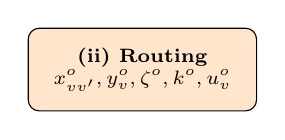
\begin{tikzpicture}[scale=0.62]
        \node[draw, rounded corners, fill=orange!20, minimum width=2.9cm, minimum height=1.05cm, align=center, font=\scriptsize] at (0,0) {\textbf{(ii) Routing}\\ $x_{vv'}^o,y_v^o,\zeta^o,k^o,u_v^o$};
      \end{tikzpicture}
      \\[0.06cm] {\tiny operations, no subtours}
    \end{column}
    \begin{column}{0.23\textwidth}
      \centering
      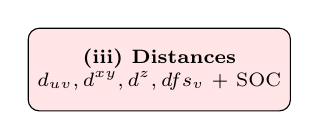
\begin{tikzpicture}[scale=0.62]
        \node[draw, rounded corners, fill=red!10, minimum width=2.9cm, minimum height=1.05cm, align=center, font=\scriptsize] at (0,0) {\textbf{(iii) Distances}\\ $d_{uv},d^{xy},d^{z},dfs_v$ + SOC};
      \end{tikzpicture}
      \\[0.06cm] {\tiny Euclidean + vertical}
    \end{column}
    \begin{column}{0.23\textwidth}
      \centering
      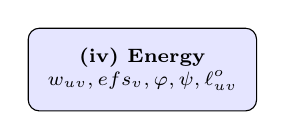
\begin{tikzpicture}[scale=0.62]
        \node[draw, rounded corners, fill=blue!10, minimum width=2.9cm, minimum height=1.05cm, align=center, font=\scriptsize] at (0,0) {\textbf{(iv) Energy}\\ $w_{uv},efs_v,\varphi,\psi,\ell_{uv}^o$};
      \end{tikzpicture}
      \\[0.06cm] {\tiny drag + endurance}
    \end{column}
  \end{columns}
  \vspace{0.18cm}
  {\small
  \[
    \min\;W=\sum_{(u,v)}\sum_{o} \ell_{uv}^o \quad\text{s.t. Loc-C,\; $D$-C,\; Dist-C,\; $w$-C,\; Endurance}
  \]
  }
  {\scriptsize $\ell_{uv}^o$ linearises $x_{uv}^o d_{uv}$ (objective) and $x_{uv}^o w_{uv}$ (endurance) via big-$M$.}
\end{frame}

% --- one family per slide ---

\begin{frame}{(i) Location constraints}
  \begin{columns}[T,onlytextwidth]
    \begin{column}{0.55\textwidth}
      {\scriptsize Vertex $v=(r,i)$ on segment $s$ of chosen chain $t$, offset $\gamma_v\in[0,1]$:}
      {\footnotesize
      \begin{align*}
        P_v &=\sum_{t,s}\bigl[\mu_v^{ts}Q^s+\eta_v^{ts}(Q^{s+1}{-}Q^s)\bigr] \tag{Loc-C$_1$}\\
        P_v^z &=\sum_{t,s}\mu_v^{ts}h_t \tag{Loc-C$_1^z$}\\
        \sum_{s}\mu_v^{ts}&=\alpha_t,\quad \sum_t\alpha_t=1 \tag{Loc-C$_{2,3}$}
      \end{align*}}
      {\scriptsize $\eta_v^{ts}=\gamma_v\mu_v^{ts}$ via Fortet. \par}
      \vspace{0.05cm}
      {\scriptsize Parametrisation $\lambda_v\in[0,S_t]$:}
      {\footnotesize
      \begin{align*}
        \lambda_v &=\sum_{t,s}(s{-}1)\mu_v^{ts}+\gamma_v \tag{Loc-C$_4$}\\
        \lambda_v &=0\;(v{=}(r,1),(r,2)) \tag{Loc-C$_5$}\\
        \lambda_v &=\sum_t S_t\alpha_t\;(v{=}(r,2R{+}1),(r,2R{+}2)) \tag{Loc-C$_8$}
      \end{align*}}
    \end{column}
    \begin{column}{0.43\textwidth}
      \centering
      
\includegraphics[width=\linewidth]{pictures/set_I.pdf}
      {\footnotesize
      \begin{align*}
        \mu_v^{t0}&=\alpha_t,\;\mu_v^{t,S_t{-}1}=\alpha_t \tag{Loc-C$_{5b,8b}$}\\
        \lambda_u&\le\lambda_v &&\!(u,v)\in\mathcal{E}_{RL}^{int} \tag{Loc-C$_6$}\\
        \lambda_u&=\lambda_v &&\!(u,v)\in\mathcal{E}_{LR}^{int} \tag{Loc-C$_7$}
      \end{align*}}
      \begin{block}{Note}
        {\scriptsize RL = forward, LR = zero-length return ($\lambda_u{=}\lambda_v$).}
      \end{block}
    \end{column}
  \end{columns}
\end{frame}

\begin{frame}{(ii) Routing constraints}
  \begin{columns}[T,onlytextwidth]
    \begin{column}{0.56\textwidth}
      {\scriptsize $x_{vv'}^o$: traverse $v{\to}v'$ in $o$; $y_v^o$: visit $v$ in $o$; $\zeta^o$: all done.}
      {\footnotesize
      \begin{align*}
        \sum_{v'}x_{v_0v'}^o &=1-\zeta^o \tag{$D$-C$_1$}\\
        \sum_{v'}x_{v'v_0}^o &=1-\zeta^o \tag{$D$-C$_3$}\\
        \sum_{v'}x_{v'v}^o-\sum_{v'}x_{vv'}^o &=0 \tag{$D$-C$_2$}\\
        \sum_{v'}x_{vv'}^o &=y_v^o,\;\sum_{v'}x_{v'v}^o=y_v^o \tag{$D$-C$_{4,5}$}\\
        \sum_o y_v^o &=1 \tag{$D$-C$_6$}\\
        \sum_o x_{vv'}^o &=1\;(v,v')\in\mathcal{E}_{RL}^{int} \tag{$D$-C$_8$}
      \end{align*}}
      {\scriptsize MTZ: $u_v^o-u_{v'}^o+1\le |\mathcal{V}'|(1-x_{vv'}^o)$\hfill (D-C$_7$)}
    \end{column}
    \begin{column}{0.42\textwidth}
      \centering
      {\small Valid inequalities}\\[0.05cm]
      {\footnotesize
      \begin{align*}
        \zeta^o &\le\zeta^{o+1} \tag{Mon.}\\
        k^o &=\sum_{v}y_v^o \tag{$k$-C}\\
        \sum_{o'<o}k^{o'} &\ge |\mathcal{V}'|\zeta^o \tag{VI-C$_1$}\\
        k^o &\ge 1-\zeta^o \tag{VI-C$_2$}
      \end{align*}}
      \begin{alertblock}{Meaning}
        {\scriptsize $\zeta^o{=}1$ $\Rightarrow$ idle operation; monotonicity removes symmetry.}
      \end{alertblock}
    \end{column}
  \end{columns}
\end{frame}

\begin{frame}{(iii) Distance constraints}
  \begin{columns}[T,onlytextwidth]
    \begin{column}{0.52\textwidth}
      {\small Intra-region (DFS trick): avoids $\beta_{vv'}^{ss'}=\mu_v^s\mu_{v'}^{s'}$}
      {\footnotesize
      \begin{align*}
        dfs_v &=\sum_{t,s}[\operatorname{cum}(s)\mu_v^{ts}+L(s)\eta_v^{ts}] \tag{DFS}\\
        d_{uv} &=dfs_v-dfs_u &&\!(u,v)\in\mathcal{E}_{RL}^{int} \tag{Dist-C$_1$}\\
        d_{uv} &=0 &&\!(u,v)\in\mathcal{E}_{LR}^{int} \tag{Dist-C$_2$}
      \end{align*}}
      {\scriptsize $dfs_v$ = cumulative distance from chain start. \par}
      \vspace{0.06cm}
      {\small Depot legs:}
      {\footnotesize
      \begin{align*}
        d_{v_0v}=d_v^{xy}+d_v^z,\; d_v^{xy}\ge\|(P_v^x,P_v^y)\|_2,\; d_v^z\ge|P_v^z| \tag{Dep-C}
      \end{align*}}
    \end{column}
    \begin{column}{0.46\textwidth}
      {\small Inter-region: $xy+z$}
      {\footnotesize
      \begin{align*}
        d_{vv'} &=d_{vv'}^{xy}+d_{vv'}^z \tag{Dist-C$_3$}\\
        d_{vv'}^{xy} &\ge\|(P_v^x,P_v^y)-(P_{v'}^x,P_{v'}^y)\|_2 \tag{Dist-C$_4$ SOC}\\
        d_{vv'}^z &\ge |P_v^z-P_{v'}^z| \tag{Dist-C$_{5,6}$}
      \end{align*}}
      \begin{block}{Key}
        {\scriptsize Dist-C$_4$ is a \textbf{second-order cone}. Both bounds tight at optimum. DFS/EFS replaces $O(|\mathcal{V}'|^2|\mathcal{S}_t|^2)$ bilinear $\beta$ variables.}
      \end{block}
    \end{column}
  \end{columns}
\end{frame}

\begin{frame}{(iv) Energy — intra-region}
  \begin{columns}[T,onlytextwidth]
    \begin{column}{0.55\textwidth}
      {\small EFS mirrors DFS:}
      {\footnotesize
      \begin{align*}
        efs_v &=\sum_{t,s}C_{ts}[\operatorname{cum}(s)\mu_v^{ts}+L(s)\eta_v^{ts}] \tag{EFS}\\
        w_{uv} &=efs_v-efs_u &&\!(u,v)\in\mathcal{E}_{RL}^{int} \tag{$w$-C$_1$}\\
        w_{uv} &=0 &&\!(u,v)\in\mathcal{E}_{LR}^{int} \tag{$w$-C$_2$}
      \end{align*}}
      {\scriptsize $C_{ts}=E^{xy}\rho_t\nu_{ts}^d$ precomputed energy per metre. \par}
      \vspace{0.08cm}
      {\small Depot legs:}
      {\footnotesize
      \begin{align*}
        w_{v_0v} &= E^{xy}\rho_0\nu^{xy}d^{xy}+\tfrac12 E^{z}\rho_0\nu^{z}d^{z}\\
        w_{vv_0} &= E^{xy}\rho_0\nu^{xy}d^{xy} \tag{no recuperation}
      \end{align*}}
    \end{column}
    \begin{column}{0.43\textwidth}
      \centering
      \begin{block}{Saving}
        {\scriptsize Same trick as DFS: exact elimination of bilinear $\mu_v^s\mu_{v'}^{s'}$; no approximation.}
      \end{block}
      \vspace{0.12cm}
      {\scriptsize $efs_v$ = cumulative energy from chain start. Ascent pays $E^{z}$, descent does not.}
    \end{column}
  \end{columns}
\end{frame}

\begin{frame}{(iv) Energy — inter-region}
  {\small With $\varphi_{rr'},\psi_{rr'}\in\{0,1\}$ (flight altitude \& vertical ordering):}
  {\footnotesize
  \begin{equation*}
    \begin{aligned}
      w_{vv'}&=\varphi_{rr'}\!\left(E^{xy}d_{vv'}^{xy}\!\sum_t\!\alpha_t\rho_t|\nu_{rr't}^d|+E^{z}\psi_{rr'}d_{vv'}^{z}\tfrac12\!\sum_\tau\!\sum_t\!\alpha_t\rho_t\nu^{z}\right)\\
      &\quad+(1-\varphi_{rr'})\!\left(E^{xy}d_{vv'}^{xy}\!\sum_t\!\alpha_t\rho_t|\nu_{rr't}^d|+E^{z}(1-\psi_{rr'})d_{vv'}^{z}\tfrac12\!\sum_\tau\!\sum_t\!\alpha_t\rho_t\nu^{z}\right)
    \end{aligned}
    \tag*{$w$-C$_3$}
  \end{equation*}}
  \vspace{0.08cm}
  \begin{columns}[T,onlytextwidth]
    \begin{column}{0.58\textwidth}
      {\scriptsize All products $\varphi\psi\alpha d$ linearised via Fortet (\texttt{\_lin\_bb}, \texttt{\_lin\_bc}), 4 constraints each.}
    \end{column}
    \begin{column}{0.40\textwidth}
      \begin{alertblock}{Complexity}
        {\scriptsize Most technical part; fully linearised.}
      \end{alertblock}
    \end{column}
  \end{columns}
\end{frame}

\begin{frame}{Endurance \& objective}
  \begin{columns}[T,onlytextwidth]
    \begin{column}{0.52\textwidth}
      {\small Endurance (big-$M$):}
      {\footnotesize
      \begin{align*}
        \ell_{uv}^o &\le x_{uv}^oM \tag{End-Lin$_1$}\\
        \ell_{uv}^o &\le w_{uv} \tag{End-Lin$_2$}\\
        \ell_{uv}^o &\ge w_{uv}-(1-x_{uv}^o)M \tag{End-Lin$_3$}\\
        \ell_{uv}^o &\ge 0 \tag{End-Lin$_4$}\\
        \sum_{u,v}\ell_{uv}^o &\le W^{\max}\;\;\forall o \tag{Endurance}
      \end{align*}}
      {\scriptsize $\ell_{uv}^o$ linearises $x_{uv}^o w_{uv}$.}
    \end{column}
    \begin{column}{0.46\textwidth}
      \begin{alertblock}{Objective}
        {\small $\min W=\sum_{u,v}\sum_o \ell_{uv}^o$, $\ell_{uv}^o$ now linearises $x_{uv}^o d_{uv}$ (same variable, both bounds).}
      \end{alertblock}
      \vspace{0.12cm}
      {\scriptsize Resulting model: \textbf{MIQP} (SOC + fully linearised bilinears).}
    \end{column}
  \end{columns}
\end{frame}

% =====================================================================
%  ALGORITHMS
% =====================================================================



\begin{frame}{Problem setup}
  \begin{itemize}
    \item 3 polygonal regions, offsets generated by uniform scaling
    \item Selected chains at heights: R0 = 15\,m, R1 = 40\,m, R2 = 65\,m
    \item Drone: front area 0.1\,m$^2$, drag coef 0.3, cruise speed 15\,m/s, vertical speed 5\,m/s
    \item Pseudo-energy model: $E = 0.5 \cdot C_d \cdot A \cdot \rho \cdot v \cdot d$ (Joules)
    \item One drone, one depot: after each operation it returns to swap the battery; endurance $W^{\max}$ caps every operation
    \item \textbf{New implementation}: the drone may enter or leave each ring \emph{at any point} of its perimeter
  \end{itemize}
  \centering
  \includegraphics[height=0.50\textheight,keepaspectratio]{../sweep_results_new/endurance_150.png}
\end{frame}

\begin{frame}{Visual guide}
  \centering
  The following snapshots show the drone's path on the 3-region instance:
  \begin{itemize}
    \item \textbf{Solid lines}: RL (coverage) edges along the chain
    \item \textbf{Dotted lines}: transitions between segments or regions
    \item \textbf{Colors}: each operation in a different color
    \item All operations start from the depot ($\triangle$) and return to it
    \item \textbf{Markers}: entry/exit points, placed freely along the rings
  \end{itemize}
  \vspace{0.2cm}
  {\small Question: how many operations does a given endurance $W^{\max}$ require, and what total distance does the drone travel?}
\end{frame}

\begin{frame}{Endurance = 150 J — 3 operations}
  \centering
  \droneAnim{150}{001}{050}
\end{frame}









\begin{frame}{Endurance = 600 J — 1 operation}
  \centering
  \droneAnim{600}{001}{048}
\end{frame}





\begin{frame}{Showcase summary}
  \centering
  \begin{tabular}{c|c|c|c}
    Endurance (J) & Operations & Distance (m) & Gap (\%) \\ \hline
    150 & 3 & 708.0 & 1.8 \\
    200 & 3 & 706.0 & 1.8 \\
    250 & 2 & 611.5 & 1.9 \\
    300 & 2 & 596.6 & 24.5 \\
    400 & 1 & 500.5 & 2.0 \\
    600 & 1 & 500.2 & 2.0
  \end{tabular}
  \vspace{0.15cm}

  {\small More endurance $\Rightarrow$ fewer depot returns $\Rightarrow$ shorter total tour.}
  \vfill
  {\footnotesize \textit{New implementation with free entry/exit points on the rings; Gurobi TL 45\,s, MIPGap 2\% (300\,J run ended at the time limit).}}
\end{frame}

% =====================================================================
%  PROBLEM & MODEL
% =====================================================================


\begin{frame}{Multi-phase heuristic: overview}
  \begin{columns}[T,onlytextwidth]
    \begin{column}{0.44\textwidth}
      \centering
      \includegraphics[width=\linewidth,height=0.62\textheight,keepaspectratio]{pictures/heuristic_flow.pdf}\\
      {\tiny 7 stages $\to$ 3 phases \par}
    \end{column}
    \begin{column}{0.54\textwidth}
      {\small Three phases:}
      \begin{enumerate}
        \item \textbf{Pre-processing}: chain selection + ring geometry
        \item \textbf{Construction}: giant tour + greedy endurance split
        \item \textbf{Improvement}: coordinate descent + 2-opt \& Or-opt
      \end{enumerate}
      \vspace{0.08cm}
      \begin{alertblock}{Goal}
        {\small Feasible solution in \textbf{$<0.6$\,s} as \textbf{warm-start} for the MIQP (10--100$\times$ faster first incumbent).}
      \end{alertblock}
    \end{column}
  \end{columns}
\end{frame}

\begin{frame}{Heuristic: phases 1--3 in detail}
  \begin{columns}[T,onlytextwidth]
    \begin{column}{0.52\textwidth}
      {\small Phase 1 -- chain selection:}
      \begin{itemize}
        \item Keep only max-resolution chains
        \item Proxy $c(t)=\sum \operatorname{perim}(\kappa)+0.5\,(d_{xy}+h_t)$ per region
      \end{itemize}
      {\small Phase 2 -- construction:}
      \begin{itemize}
        \item Nearest-neighbour on 3D centroids from $v_0$; expand rings interior$\to$exterior
        \item Greedy split: add rings while energy $\le W^{\max}$, else close operation
      \end{itemize}
    \end{column}
    \begin{column}{0.46\textwidth}
      {\small Phase 3 -- improvement:}
      \begin{itemize}
        \item Entry-point coordinate descent (60 samples, 8 passes)
        \item \textbf{2-opt} intra-operation; \textbf{Or-opt} inter-operation (relocate ring if both ops feasible and energy drops)
        \item Final solution feeds Gurobi \texttt{Start} (\texttt{set\_warm\_start})
      \end{itemize}
      \vspace{0.08cm}
      {\scriptsize $\gamma=0.5$, $N_{\rm samples}=60$, $N_{\rm coord}=8$, $N_{\rm passes}^{\rm op}=10$.}
    \end{column}
  \end{columns}
\end{frame}

% =====================================================================
%  EXPERIMENTS — MEANS FROM AVAILABLE DATA
% =====================================================================

\begin{frame}{Experimental design}
  \begin{columns}[T,onlytextwidth]
    \begin{column}{0.52\textwidth}
      {\small Testbed:}
      \begin{itemize}
        \item $n_r\in\{1,2,3,5,8,10\}$ $\times$ 3 height levels $\times$ 5 seeds $\times$ 6 endurance values $=$ \textbf{540 configs}
        \item Methods: heuristic ($H$), Vertex-Approach MIQP cold ($R$), warm-started ($R{+}WS$)
        \item Heights: L1 \{30\}, L2 \{20,50\}, L3 \{15,35,60\}\,m
      \end{itemize}
      {\scriptsize \textbf{Status (31 Aug 2026):} Vertex-Approach sweep complete — 540 configs $\times$ 3 methods = 1620 runs (1703 CSV rows).}
    \end{column}
    \begin{column}{0.45\textwidth}
      {\small Endurance calibration:}
      {\scriptsize cheapest single-region tour; rounded to 300\,J (5\% margin).}
      {\tiny
      \begin{tabular}{lrr}
        \toprule Factor & Raw & Rounded\\\midrule
        $E_{\min}$ & 245.9 & --\\
        1.0 & 300 & 300\\ 1.5 & 450 & 450\\ 2.0 & 600 & 600\\
        3.0 & 900 & 900\\ 5.0 & 1500 & 1500\\ 8.0 & 2400 & 2400\\\bottomrule
      \end{tabular}}
      \\[0.05cm]
      {\scriptsize Solver: Gurobi 11.0, MIPGap=0, TL=1800\,s, 1 thread. \par}
      {\scriptsize All means below computed from \texttt{compare\_results/results.csv}.}
    \end{column}
  \end{columns}
\end{frame}

\begin{frame}{Results — aggregated means (vertex, complete)}
  \centering
  {\scriptsize \begin{table}[t]
\centering
\caption{Aggregated results for the Vertex-Approach (MTZ) formulation. Mean objective and solve time averaged over height levels ($n_h=1,2,3$), endurance levels ($E=300$--2400\,J) and 5 seeds. MIP gap at the 1800\,s limit. $H$ = heuristic standalone.}
\label{tab:results-summary-rings}
\resizebox{\textwidth}{!}{%
\begin{tabular}{crrrrrrrr}
\toprule
$n_r$ & \multicolumn{2}{c}{$H$} & \multicolumn{3}{c}{$R$ (Vertex-Approach)} & \multicolumn{3}{c}{$R$+WS (Vertex-Approach+WS)} \\
\cmidrule(lr){2-3} \cmidrule(lr){4-6} \cmidrule(lr){7-9}
 & Obj. & Time (s) & Obj. & Time (s) & Gap (\%) & Obj. & Time (s) & Gap (\%) \\
\midrule
1 & 206.5 & 0.03 & 201.6 & 85.1 & 0.1 & 202.0 & 86.9 & 0.1 \\
2 & 375.0 & 0.06 & 364.3 & 454.3 & 4.2 & 363.8 & 436.6 & 4.0 \\
3 & 517.0 & 0.10 & 485.9 & 1088.8 & 8.0 & 485.8 & 1094.0 & 8.3 \\
5 & 989.2 & 0.21 & 992.4 & 1790.3 & 26.0 & 943.4 & 1800.1 & 23.9 \\
8 & 1676.2 & 0.41 & 2163.7 & 1800.2 & 49.9 & 1647.5 & 1800.2 & 37.8 \\
10 & 2175.2 & 0.54 & 3283.6 & 1800.3 & 61.3 & 2017.2 & 1800.3 & 42.2 \\
\bottomrule
\end{tabular}%
}
\end{table}
}
  {\tiny Means over $n_h$, $E$, seeds (540 configs). $H$ = heuristic; $R$ = vertex MIQP; $R{+}WS$ = warm-started. \par}
  \vspace{0.1cm}
  {\scriptsize \textbf{Read:} gap 0.1\% at $n_r=1$ (optimality proven) $\to$ 61\% at $n_r=10$ cold, 42\% warm. Heuristic $0.03$--$0.54$\,s always feasible.}
\end{frame}



\begin{frame}{Results — endurance effect ($n_r=3$, means)}
  \centering
  {\scriptsize \begin{table}[t]
\centering
\caption{Effect of endurance $E$ for $n_r=3$ (averaged over $n_h=1,2,3$ and 5 seeds). Tight $E$ implies more operations and higher total distance.}
\label{tab:results-by-endurance}
\resizebox{\textwidth}{!}{%
\begin{tabular}{crrrrrrrr}
\toprule
$E$ (J) & \multicolumn{2}{c}{$H$} & \multicolumn{3}{c}{$R$} & \multicolumn{3}{c}{$R$+WS} \\
\cmidrule(lr){2-3} \cmidrule(lr){4-6} \cmidrule(lr){7-9}
 & Obj. & Time & Obj. & Gap & Time & Obj. & Gap & Time \\
\midrule
300 & 570.8 & 0.10 & 524.7 & 9.5 & 1122.7 & 525.8 & 9.5 & 1066.8 \\
450 & 528.3 & 0.10 & 492.2 & 9.7 & 1121.8 & 492.2 & 10.8 & 1120.2 \\
600 & 500.7 & 0.09 & 474.3 & 6.5 & 1062.7 & 474.3 & 7.6 & 1143.7 \\
900 & 500.7 & 0.09 & 474.5 & 7.5 & 1070.7 & 474.3 & 7.4 & 1110.3 \\
1500 & 500.7 & 0.10 & 475.2 & 7.0 & 1037.1 & 474.3 & 7.4 & 1035.5 \\
2400 & 500.7 & 0.10 & 474.5 & 8.1 & 1117.7 & 474.3 & 7.1 & 1087.4 \\
\bottomrule
\end{tabular}%
}
\end{table}
}
  {\tiny $n_r=3$ fixed, averaged over $n_h$ and seeds. \par}
  \vspace{0.08cm}
  {\scriptsize Tight $E=300$ $\Rightarrow$ $\approx$525\,m; $E\ge600$ $\Rightarrow$ $\approx$474\,m (endurance-unconstrained plateau). Same conclusion as the 60--120\,J showcase, now on 90 instances.}
\end{frame}

\begin{frame}{Comparative figures — time \& gap}
  \begin{columns}[T,onlytextwidth]
    \begin{column}{0.50\textwidth}
      \centering
      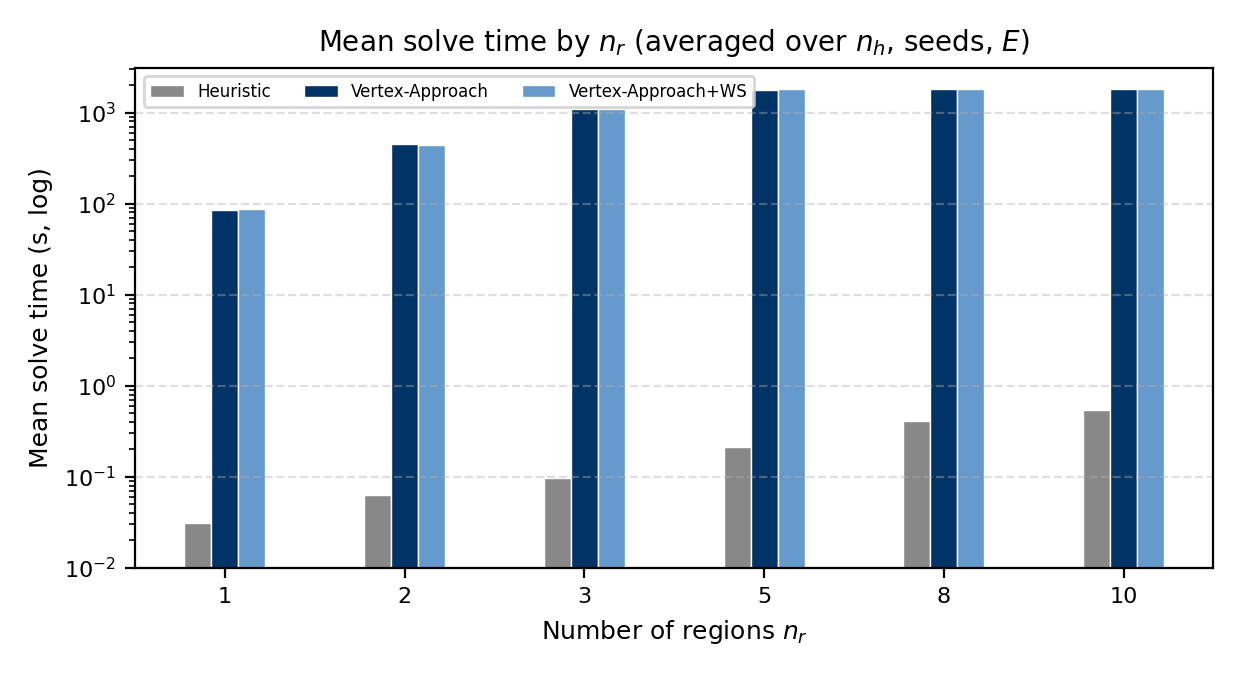
\includegraphics[width=\linewidth]{pictures/compare_time_by_regions_vertex.pdf}\\
      {\tiny Log scale \par}
    \end{column}
    \begin{column}{0.50\textwidth}
      \centering
      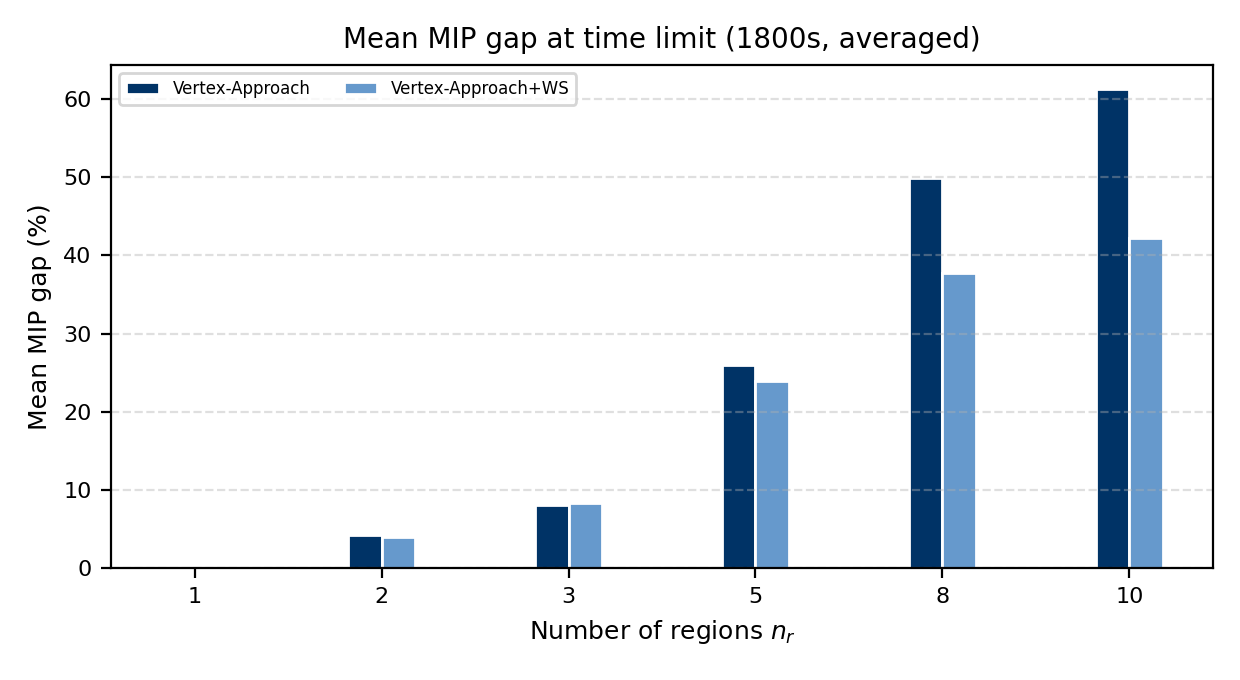
\includegraphics[width=\linewidth]{pictures/compare_gap_by_regions_vertex.pdf}\\
      {\tiny Gap at 1800\,s; warm-start clearly reduces gap for large $n_r$ \par}
    \end{column}
  \end{columns}
\end{frame}

\begin{frame}{Warm-start benefit \& visual solutions}
  \begin{columns}[T,onlytextwidth]
    \begin{column}{0.50\textwidth}
      \centering
      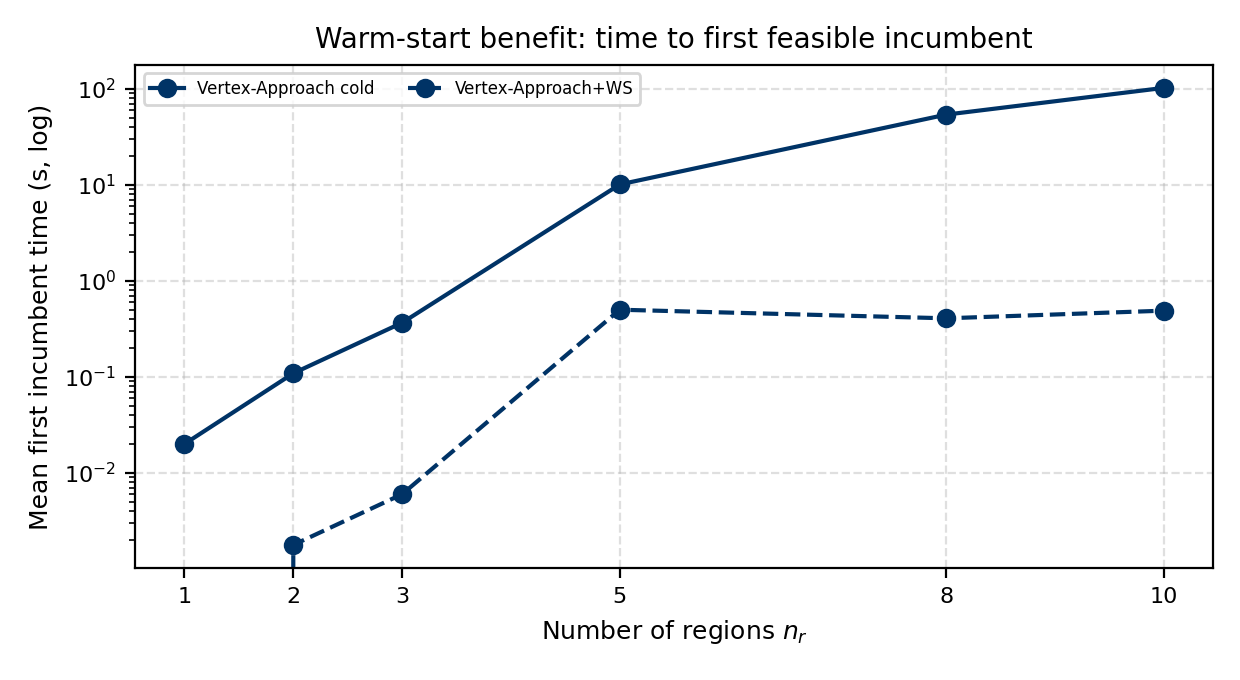
\includegraphics[width=\linewidth]{pictures/compare_first_incumbent_vertex.pdf}\\
      {\tiny Time to first feasible incumbent, $n_r=1..10$ (mean over seeds/$n_h$/$E$); dashed = warm-start \par}
    \end{column}
    \begin{column}{0.48\textwidth}
      \centering
      \includegraphics[width=0.92\linewidth]{../solution_2h.png}\\
      {\tiny 2 regions, 2 altitudes; colour = operation \par}
      \vspace{0.08cm}
      \includegraphics[width=0.92\linewidth]{../solution_5r.png}\\
      {\tiny 5 regions; heuristic avoids crossings, MIQP refines \par}
    \end{column}
  \end{columns}
  \vspace{0.06cm}
  {\scriptsize Warm-start saves 10--100$\times$ to the first feasible incumbent, most for tight endurances.}
\end{frame}

% =====================================================================
%  CLOSE
% =====================================================================


\begin{frame}{Vertex-Approach analysis — the complete case}
  \centering
  {\small \textbf{540 configs $\times$ 3 methods = 1620 runs, all completed (31 Aug 2026).}}
  \vspace{0.1cm}
  \begin{columns}[T,onlytextwidth]
    \begin{column}{0.54\textwidth}
      \begin{itemize}
        \item \textbf{Optimality}: gap $\approx$0.1\% for $n_r{=}1$ (proven); $n_r{\le}3$ within $\approx$8\% at the 1800\,s limit
        \item \textbf{Heuristic}: 0.03--0.54\,s, \emph{always} feasible, within 2--6\% of the exact objective on provable instances
        \item \textbf{Warm-start}: 10--100$\times$ faster to the first feasible incumbent; final gap at $n_r{=}10$ drops 61\% $\to$ 42\%
      \end{itemize}
    \end{column}
    \begin{column}{0.44\textwidth}
      \begin{itemize}
        \item \textbf{Endurance effect} ($n_r{=}3$): $E{=}300$\,J $\Rightarrow$ $\approx$525\,m vs $E{\ge}600$\,J $\Rightarrow$ $\approx$474\,m; plateau $\Rightarrow$ endurance-unconstrained
        \item \textbf{Scalability}: solve time grows with $n_r$; all $n_r{\ge}5$ hit the time limit, WS recovers $\approx$10--20\% gap
      \end{itemize}
    \end{column}
  \end{columns}
  \vspace{0.1cm}
  {\scriptsize All means from \texttt{compare\_results/results.csv} (\texttt{table\_results\_summary}, \texttt{table\_results\_by\_endurance}, \texttt{compare\_*\_vertex}).}
\end{frame}

\begin{frame}{Conclusions \& future work}
  \begin{columns}[T,onlytextwidth]
    \begin{column}{0.58\textwidth}
      {\small Contributions:}
      \begin{enumerate}
        \item MIQP with \textbf{preemption + altitude + endurance} in one model (SOC + big-$M$), one family per slide
        \item Equivalent \textbf{edge-based} DFJ reformulation
        \item Multi-phase heuristic $<0.6$\,s that \textbf{warm-starts} the exact solver
        \item Mean-based results on the full 540-config Vertex-Approach sweep
      \end{enumerate}
      \vspace{0.1cm}
      {\small Future:}
      \begin{itemize}
        \item Multi-drone heterogeneous fleet; dynamic wind
        \item VNS/LNS metaheuristics; real missions
      \end{itemize}
    \end{column}
    \begin{column}{0.40\textwidth}
      \centering
      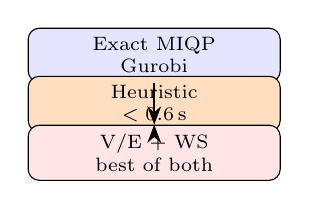
\begin{tikzpicture}[scale=0.62, every node/.style={font=\scriptsize}]
        \node[draw, rounded corners, fill=blue!10, minimum width=3.2cm, minimum height=0.65cm, align=center] (a) at (0,2.0) {Exact MIQP\\ Gurobi};
        \node[draw, rounded corners, fill=orange!25, minimum width=3.2cm, minimum height=0.65cm, align=center] (b) at (0,1.0) {Heuristic\\ $<0.6$\,s};
        \node[draw, rounded corners, fill=red!10, minimum width=3.2cm, minimum height=0.65cm, align=center] (c) at (0,0) {V/E + WS\\ best of both};
        \draw[-{Stealth}, thick] (b) -- (c);
        \draw[-{Stealth}, thick] (a) -- (c);
      \end{tikzpicture}
      \\[0.1cm]
      {\scriptsize \texttt{python compare\_methods.py --resume}\\[0.05cm]
      {\tiny Data: \texttt{compare\_results*/results.csv} + \texttt{solutions/}}}
    \end{column}
  \end{columns}
\end{frame}

\begin{frame}
  \centering
  \vspace{0.4cm}
  {\Huge Thank you!}\\[0.2cm]
  {\large Coverage Path Planning}\\[0.1cm]
  {\normalsize Impact of drone endurance on multi-operation planning}\\[0.4cm]
  {\small Lavinia Amorosi \;$\cdot$\; Paolo Dell'Olmo \;$\cdot$\; Justo Puerto \;$\cdot$\; \textbf{Carlos Valverde}}\\[0.08cm]
  {\scriptsize University of Seville -- Sapienza University of Rome \par}
  \vspace{0.4cm}
  {\small \textbf{Questions?}}\\[0.15cm]
  {\scriptsize \texttt{cvalverde@us.es} \;\textperiodcentered\; \texttt{github.com/z72vamac/drone-cpp} \;\textperiodcentered\; \texttt{articulo/main.tex}}\\[0.1cm]
  {\tiny \color{gray} Talk designed for 15--17\,min. Slides in English, presentation in Spanish. \par}
\end{frame}

% =====================================================================
\end{document}